\section{Introduction} 

Assistive exoskeletons are a growing field of study. Systems like the Rewalk \cite{esquenazi2012rewalk}, Esko \cite{mertz2012next}, and Vanderbilt exoskeletons \cite{gasser2017design} have presented promising results; their systems enable people with spinal cord injuries (SCI) and other neurological conditions to stand and walk with assistance \cite{farris2013preliminary}. The trajectory generation is essential so that joints follow natural motions. The lower level motion controller handles the variation of the mass of the person and the contact dynamics. Exoskeletons directly interface with a person's body. The joint movement control closely follows the user’s natural joint movement; if this motion does not appropriately match the user's joint motion, then there is an excess strain on the person’s joints.

The exoskeleton should move in an anatomically correct manner. Both walking and stair climbing are activities of daily living (ADL). Stair climbing is considered a hazardous form of locomotion \cite{HicksLittle2011LowerEJ}  due to the potential for the foot to collide with the stair if the trajectory is incorrect.  

Two fields of research in lower-limb exoskeleton control are the controller's design and the trajectory controller \cite{huang2016optimisation}. These two fields are highly related; the controller produces the torques, while the trajectory generation moves the joints and ensures that the placement of the foot is in a stable position. There is a significant amount of work on detailing how to teach a robotic system how to walk. Teaching a robot to follow a task is challenging; it involves balancing leg trajectory generation, single-leg support, and double-leg support.

Additionally, in \cite{taskjointmocap}, Hu \textit{et. al} focused on online generations of trajectories. They formulated the control problem as a Quadratic Programming (QP) problem, and the authors used both Cartesian and joint data as the imitation criteria. The formulation as a QP problem allows for inequality and equality constraints for the knee velocity. This formulation resolves the conflicts between the joint space and the Cartesian imitation data. This method is limited to level ground walking. This process did not address the problem of abstracting the trajectories for different stair heights; it only addresses level ground walking and fully actuated systems.

Able-bodied people have the innate ability to adapt and adjust to their environment. When they encounter stairs of different heights, they can ascend them without issue. For exoskeletons to climb stairs, they need to have the same ability to adapt to different stair heights. This paper presents a model to allow exoskeletons to adapt their motion to different stair heights. The motion capture system (mocap) records joint kinematics during stair ascent to build a library.

Stair climbing is a non-linear task that engages multiple muscle groups and requires balancing the torso. Ascending stairs requires one foot to remain on the ground while the other foot swings through a trajectory\cite{hicks2012temporal}. Several studies have examined how people climb upstairs. Motion capture is one tool that can be used for recording human kinematics and kinetics. In  \cite{chalodhorn2007learning}, Chalodhorn \textit{et. al} used a model-free approach to teach a robot to walk.
In  \cite{hu2014online}, Hu \textit{et. al} used quadratic programming to optimize the mapping of the markers to the robot. In both cases, the motion capture mapping was mapped from a human to a humanoid robot. Although exoskeletons and biped robots share many similarities, exoskeletons have additional constraints. They have to interface with a person who imposes the joint biological limits on the system. The exoskeleton joints have to be co-linear with the person and avoid skin irritation. These constraints should be considered when designing a controller for a lower limb exoskeleton. The exoskeleton has to comply with human movement.

The work conducted in \cite{andriacchi1980study} and \cite{hicks2011lower} focused on the kinematics and dynamics of stair climbing by using a combination of motion capture, force plates, and IMUs sensors. These studies have produced high-resolution joint angle data for level ground walking and stair climbing.

%\subsection{Learning from Demonstration}  

Learning from Demonstration (LfD) is the process of transferring skills to a robot by demonstration. In \cite{siciliano2016springer}  \cite{kormushev2011imitation} \cite{calinon2007teacher} Calinon \textit{et al} outline the process of teaching a robot how to follow a trajectory. There are several steps in LfD: demonstration modality, motion primitives, and encoding methods. There are several steps in the LfD process, as stated below. 

\begin{enumerate}
    \item Recognition of the task 
    \item Encoding of the motion 
    \item Retrieval of the task 
    \item Reproduction of task 
\end{enumerate} 

The following two teaching modalities could be used to teach a  robot to follow a trajectory. The first teaching modality is kinesthetic teaching. This modality involves a user moving a robot passively or running an impedance controller through a task while recording the joint positions and torques \cite{Calinon2018}. Researchers have applied kinetic teaching for upper limb robotic systems for industry and human-robot interfaces. While this method is a natural method of teaching, it is not well suited for teaching lower limb movement because it would require directly moving a leg through a gait motion. It would be difficult to replicate the leg's motion by the manual moving of a person or robot. 

The other teaching modality is visual observation. In this teaching modality, visual sensors record the desired motions and intentions of a demonstration for mapping onto a robotic system \cite{CalinonLee19}. In visual observation, mocap is the standard method. The marker system allows for precise tracking of points on a person with millimeter accuracy \cite{ott2008motion}. Due to its wide adaptation and high accuracy for gait data collection\cite{ViconGaiting}, it is the method of data recording used in this paper. This paper will demonstrate a method of using lower body mapping and recognition. 

Dynamic Motion Primitives (DMPS) are a method of breaking down demonstrations into their fundamental building blocks. Motion primitives aim to encode trajectories into building blocks that can then be rearranged and manipulated. DMP are a popular form of motion primitives \cite{ijspeert2013dynamical}. They work by creating a stable underlying model and generating a forcing function to drive the system.  

In the classical formulation of DMPs, the model places radial basis functions (RBF) along the trajectory that pull the system towards the goal. DMPs are considered one of the gold standards of learning and replicating human motion \cite{nakanishi2004learning}. 

There are several LfD methods for learning trajectories, including Gaussian Mixed Regression (GMR), Hidden Markov Models (HMM), and Locally Weighted Regression (LWR). They are all methods of encoding motion into basis functions for learning and reproduction. The methods are similar but contain their pros and cons. LWR is the simplest method, with GMR and HMM being extensions. GMM and HMM place the RBF on the trajectory more effectively.  

GMR provides a more comprehensive approach to the RBF placement and allows for the encoding of multiple trajectories, while DMP is limited to a single demonstration for training. In GMR, the demonstrations are encoded using Gaussian Mixture Models (GMM)\cite{calinon2013compliant} \cite{Statisticaldynamical}. The demonstration for training the model must be temporally scaled using Dynamic time warping (DTW). GMR is computationally fast and produces smooth and continuous trajectories. The benefits of using GMR are the following \cite{Calinon}: 

\begin{enumerate}  
    \item Allows encoding of local correlation between motion variables   
    \item Provides a principled approach to estimate the parameters of the radial base functions (RBF) 
    \item Reduce the number of RBF   
    \item Online estimation of the DMP parameters and model selection   
\end{enumerate}  

Hidden Markov Models (HMM) combines temporal scaling and transition probabilities through a double stochastic process \cite{calinon2007learning}. HMM offers several benefits over the GMR method. HMM has built-in temporal scaling, meaning that it can deal with demonstrations that are not aligned. As stated by Calinon \textit{et. al}, the double stochastic process makes it difficult to retrieve smooth and continuous trajectories. It is desirable to have smooth and continuous trajectories for exoskeletons. There are four steps for building the imitation model listed below. \autoref{fig:demostation} illustrates the workflow for training and reproduction.

\begin{enumerate}
    \item Collection of gait data
    \item Encoding of motion into radial basis functions (RBF)
    \item Learning of regression function
    \item Reproduction, and manipulation of the trajectories
\end{enumerate}


To collect the necessary data for reproduction, a motion capture trial was conducted, producing a set trajectory for learning. The trajectories were extracted and segmented. The marker represents the footpath over the step motion; inverse kinematics then calculate the joint angles. This structure allows the imitation model to handle people of different heights.

Using Gaussian Mixed Model (GMM), the trajectories were encoded into RBF, placed throughout the data set. The forcing function is found using Gaussian Mixed Regression (GMR), which regresses over the RBFs. This forcing function is then used to drive the Dynamic motion primitives (DMP) model. This procedure allows for manipulation for temporal, start, and goal manipulation.  

\begin{figure} 
    \centering 
    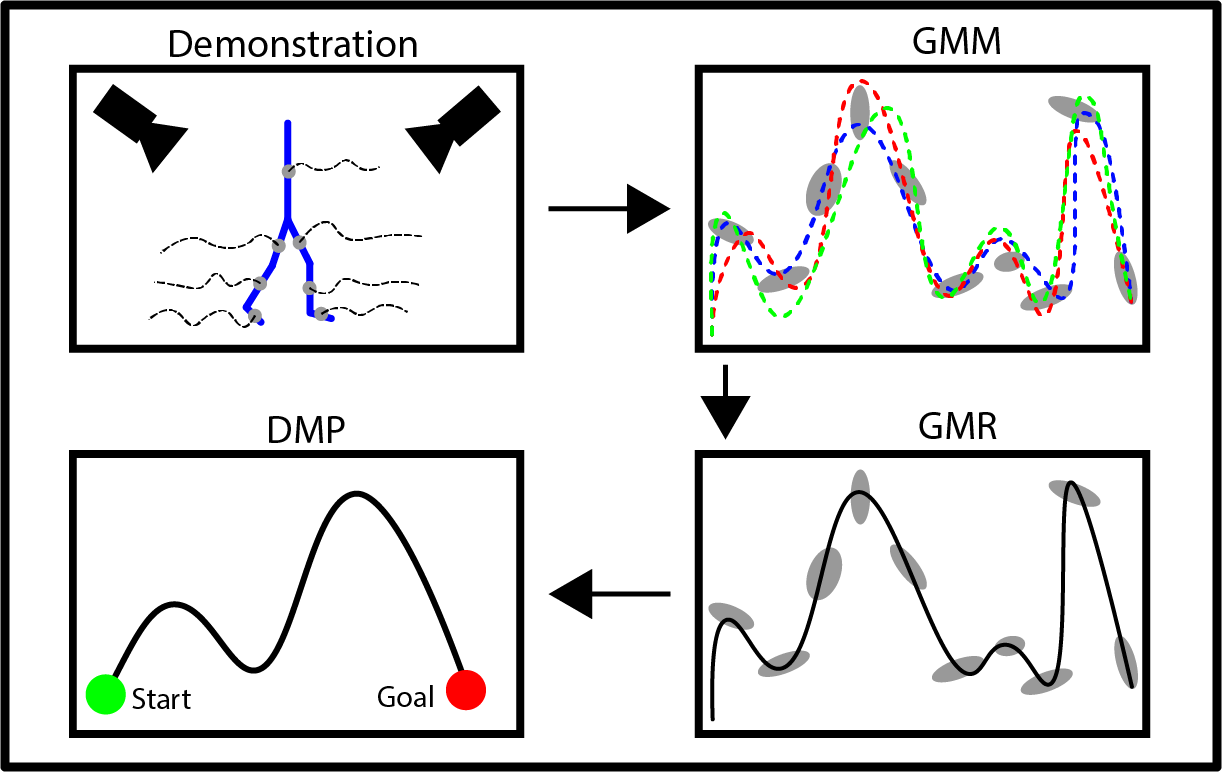
\includegraphics[scale=0.2]{images/demo_figure.png} 
    \caption{Order of operations of the learning process. The data is collected, the demos are encoded, the model is retrieved, then the model is reproduced.} 
    \label{fig:demostation} 
\end{figure} 


To increase the data in the community, all data used is available online\footnote{\url{https://github.com/WPI-AIM/AIM\_GaitData}}. This paper uses this data to train an imitation model by using Gaussian Mixed Models (GMM) for encoding and Gaussian Mixed Regression (GMR) extraction of the motion primitives and Dynamic Motion Primitives (DMPs) for manipulating the start and goal of the trajectories. This model will not need to be retrained for each individual and allows for stair height adaption.